\documentclass[11pt,a4paper]{article}

% ============================================================
% Packages
% ============================================================
\usepackage[margin=2.6cm]{geometry}
\usepackage{amsmath,amssymb,amsthm,mathtools,bm}
\usepackage{booktabs}
\usepackage{microtype}
\usepackage{xcolor}
\usepackage[most]{tcolorbox}
\usepackage{hyperref}
\usepackage{enumitem}
\usepackage{graphicx}
\usepackage{float}
\usepackage{caption}

\hypersetup{
  colorlinks=true,
  linkcolor=blue!55!black,
  citecolor=blue!55!black,
  urlcolor=blue!55!black
}

% Compiled from inside "paper figures/3 tragets source perpendicular/";
% "./" covers the sibling PNGs generated by gamma_effect_density.py,
% beta_effect.py, geometry_effect.py and phase_portrait.py.
\graphicspath{{./}}

% ============================================================
% Theorem environments (matching the companion notes)
% ============================================================
\theoremstyle{plain}
\newtheorem{theorem}{Theorem}[section]
\newtheorem{proposition}[theorem]{Proposition}
\newtheorem{lemma}[theorem]{Lemma}
\newtheorem{corollary}[theorem]{Corollary}

\theoremstyle{definition}
\newtheorem{definition}[theorem]{Definition}

\theoremstyle{remark}
\newtheorem{remark}[theorem]{Remark}

\newtcolorbox{keybox}[1][]{
  colback=gray!5, colframe=black!45, boxrule=0.7pt, arc=2pt,
  left=8pt,right=8pt,top=6pt,bottom=6pt,
  fonttitle=\bfseries, title={#1}
}
\newtcolorbox{warningbox}[1][]{
  colback=red!3, colframe=red!45, boxrule=0.7pt, arc=2pt,
  left=8pt,right=8pt,top=6pt,bottom=6pt,
  fonttitle=\bfseries, title={#1}
}

% ============================================================
% Commands (same conventions as axial_fixed_point.pdf / bandwidth_pareto_flow.tex:
% bw = beta = bandwidth, gamma = shape exponent, kernel p(d) = exp(-bw*d^gamma))
% ============================================================
\newcommand{\bx}{\bm{x}}
\newcommand{\ba}{\bm{a}}
\newcommand{\R}{\mathbb{R}}
\newcommand{\lam}{\lambda}
\newcommand{\bw}{\beta}
\newcommand{\bwc}{\beta_c}
\newcommand{\gc}{\gamma_c}
\newcommand{\de}{d_e}
\newcommand{\dth}{d_3}

\title{\bfseries
Beyond $z_c$: The Transverse Instability Strengthens\\
Past the ``Unstable Everywhere'' Boundary\\
\large Addendum to Section 12 of the Perpendicular-Geometry Companion Note
}
\author{Amit Alper\\
\small Hebrew University of Jerusalem}
\date{\today}

\begin{document}
\maketitle

\begin{abstract}
Section 12 of the companion note (\emph{axial\_fixed\_point.pdf}) shows that
in the perpendicular three-target geometry, the critical height $z_c$ at
which a descending population commits sideways to the base pair
$\{\ba_1,\ba_2\}$ moves monotonically toward the source as either the shape
exponent $\gamma$ or the bandwidth $\bw$ increases, and diverges at a
critical curve $\gc(\bw,e)$ (equivalently $\bwc(\gamma,e)$) beyond which the
axis is transversally unstable \emph{everywhere} ($z_c\to 0^-$ by
convention). Simulations at fixed source depth $h$ show something the
sign-based $z_c$ story cannot, by itself, explain: the visible fan-opening
keeps creeping toward the source as $\gamma$ (or $\bw$) increases even after
$z_c$ has already saturated at $0$ for every value in the sweep. We show
this is not a numerical artefact: the transverse eigenvalue $\lam_x(z)$
grows \emph{pointwise, monotonically and without bound} in $\gamma$ (and,
past its own threshold, in $\bw$) at every fixed height $z$ on the path --
not only at the height where it changes sign. We make this precise
(Proposition~\ref{prop:pointwise}), connect it to the visible split height
via an accumulated-growth argument (Proposition~\ref{prop:threshold}), give
the exact algebraic reason $\bw$ and $\gamma$ act differently
(Section~\ref{sec:beta_vs_gamma}), and present phase portraits
(Figure~\ref{fig:phase_portrait}) that visualise instability
\emph{strength}, not just its sign, across the $(\gamma,\bw)$ plane.
\end{abstract}

\tableofcontents

% ================================================================
\section{Setup (recap)}
% ================================================================

Geometry and notation follow Section 12 of the companion note exactly. Base
half-spacing $b=1$; archetypes
\[
\ba_1=(-b,0,0),\quad \ba_2=(b,0,0),\quad \ba_3=(0,e,0),
\]
source at $(0,e/3,-h)$ on the centroid line, population descending along
$(x,y,z)=(0,e/3,z)$, $z\in(-h,0)$. Kernel $p(d)=e^{-\bw d^\gamma}$. On the
centroid line,
\[
\de(z):=\sqrt{b^2+(e/3)^2+z^2},\qquad \dth(z):=\sqrt{(2e/3)^2+z^2},
\]
and the transverse eigenvalue along that line (eq.~13 of the companion
note; implemented verbatim in \texttt{perpendicular\_common.lambda\_x}) is
\begin{equation}
\lam_x(z;\gamma,\bw)
= \frac{2\bw^2\gamma^2}{N}\,\de^{2\gamma-4}
 -\frac{2\bw\gamma(\gamma-2)}{N}\,\de^{\gamma-4}
 -\frac{2\bw\gamma}{N}\,\de^{\gamma-2}
 -\frac{\bw\gamma}{N}\,\dth^{\gamma-2}.
\label{eq:lamx}
\end{equation}
$z_c:=\sup\{z<0:\lam_x(z)=0\}$, with $z_c=-\infty$ if $\lam_x<0$ throughout
(trapped) and $z_c\to 0^-$ if $\lam_x>0$ throughout (unstable everywhere).

\begin{keybox}[What this note adds]
Everything in the companion note's Section 12 is a statement about the
\emph{sign} of $\lam_x(z)$. Once $\gamma$ or $\bw$ pass their critical
value, $z_c$ stops moving (it is pinned at $0$) and can no longer
distinguish, say, $\gamma=2$ from $\gamma=3$ -- yet simulations
(Figure~\ref{fig:motivating}) visibly keep splitting earlier. This note
extends the theory to the \emph{magnitude} of $\lam_x(z)$, which keeps
distinguishing them.
\end{keybox}

\begin{figure}[H]
\centering
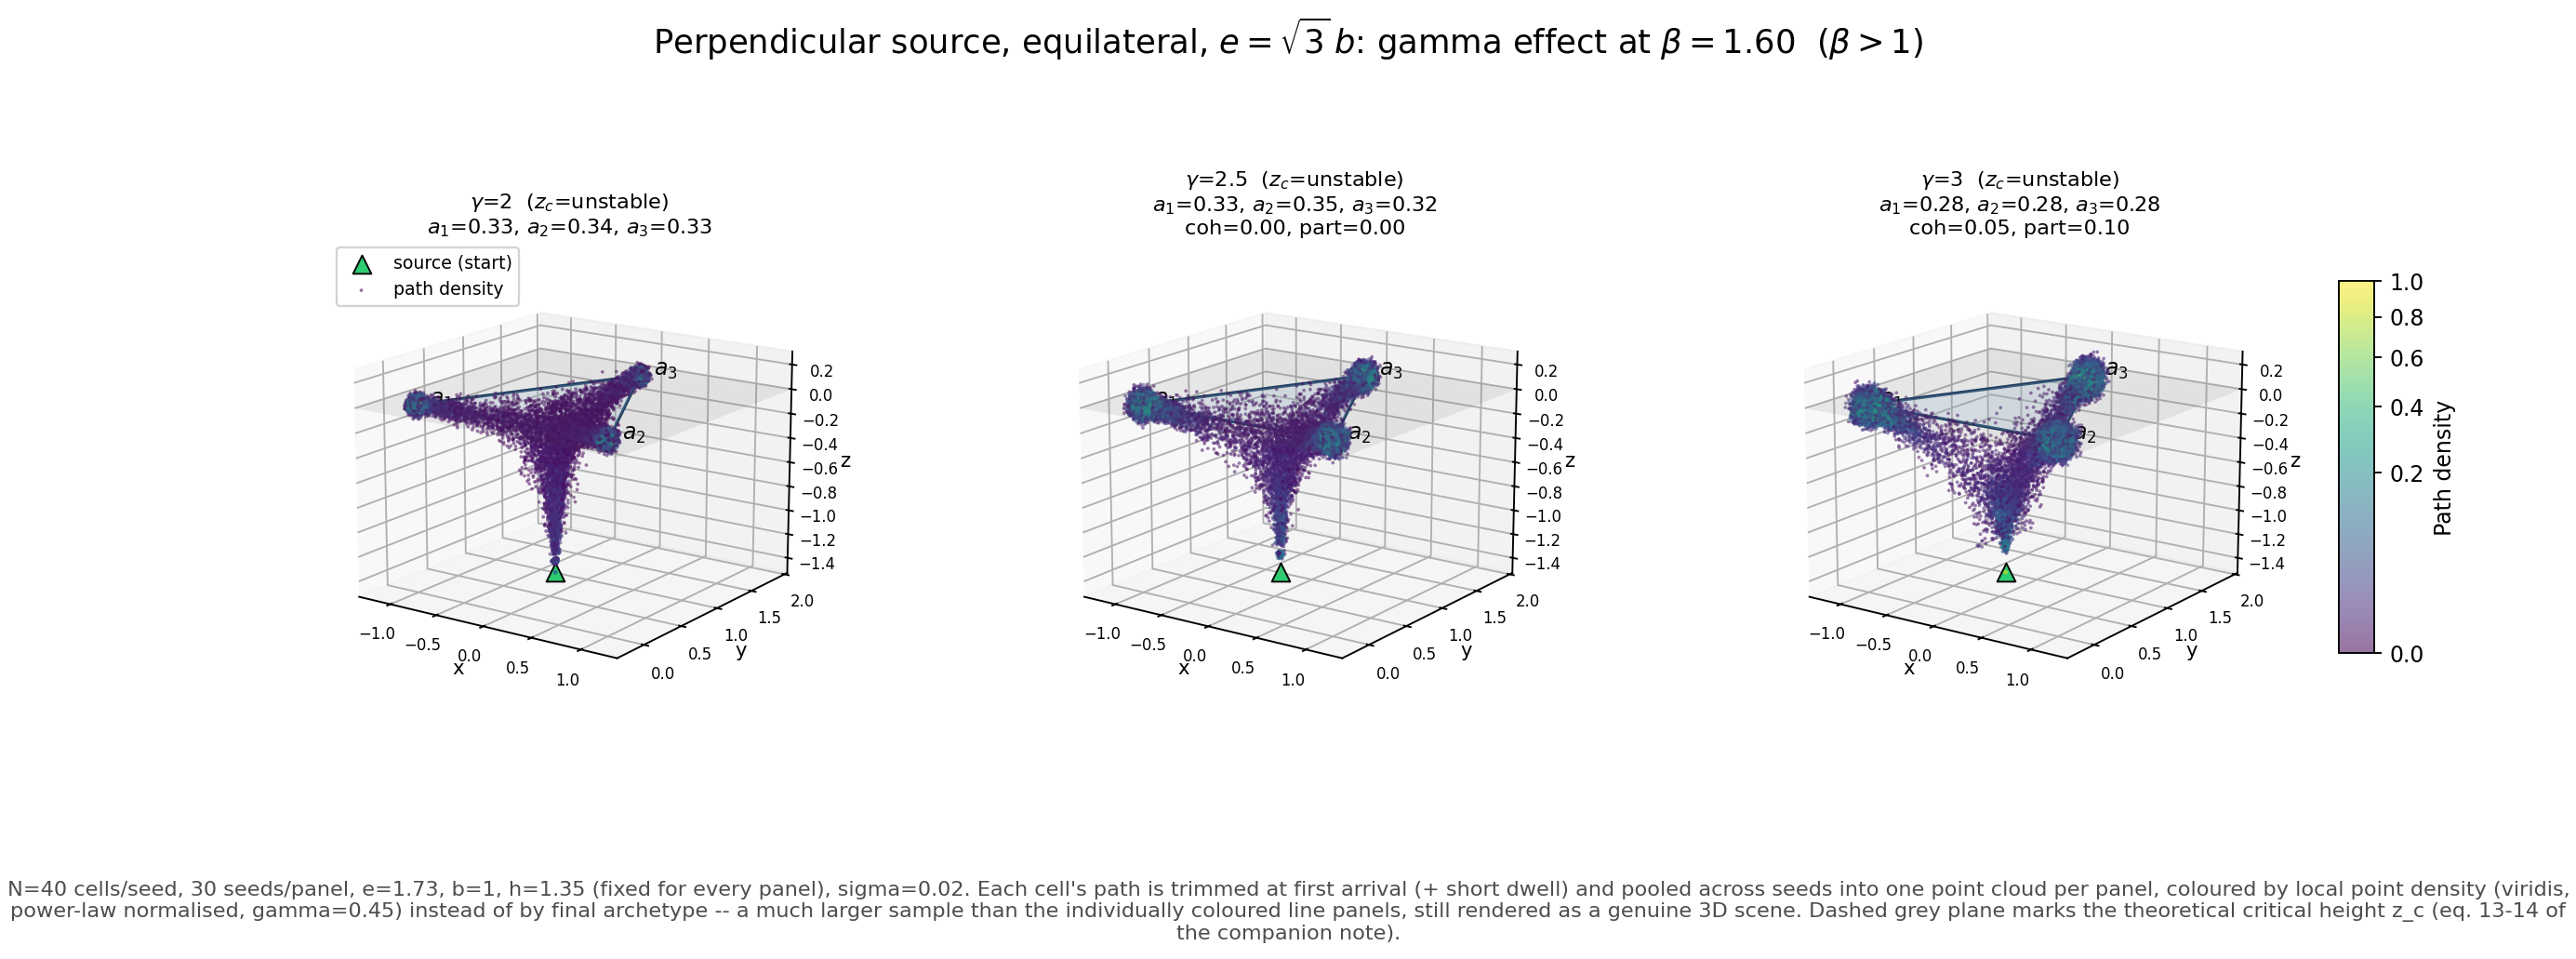
\includegraphics[width=0.95\linewidth]{gamma_effect_beta_gt1_equilateral.png}
\caption{Motivating observation: $\bw=1.60$ ($\bw>1$), equilateral
triangle, $h=1.35$. $z_c$ is finite only for $\gamma=1.2$; for
$\gamma=2,2.5,3$ the theory already says ``unstable everywhere,'' yet the
coherent trunk near the source visibly shortens further as $\gamma$
continues to grow.
\emph{(paper figures/3 tragets source perpendicular/gamma\_effect\_density.py)}}
\label{fig:motivating}
\end{figure}

% ================================================================
\section{The instability strengthens pointwise, not just at its zero}
% ================================================================

\begin{proposition}[Pointwise, unbounded monotonicity in $\gamma$]
\label{prop:pointwise}
Fix $z$, $e>0$, $b>0$, $\bw>0$. Then $\de(z)>1\ge b$ whenever $e>0$ or
$z\neq0$ (and $\de(z)\ge b=1$ always), so $\ln\de(z)>0$ on the whole open
path $z\in(-h,0)$. Consequently the leading term of \eqref{eq:lamx},
\[
\frac{2\bw^2\gamma^2}{N}\,\de(z)^{2\gamma-4}
=\frac{2\bw^2\gamma^2}{N}\exp\!\big[(2\gamma-4)\ln\de(z)\big],
\]
grows without bound as $\gamma\to\infty$ and dominates every other term in
\eqref{eq:lamx} (each of which grows at most like $\de^{\gamma}$ or
$\dth^\gamma$, i.e.\ at half the exponential rate in $\gamma$). Hence there
exists $\gamma^\dagger(z,\bw,e)$ such that
\[
\frac{\partial\lam_x}{\partial\gamma}(z;\gamma,\bw)>0
\qquad\text{for all } \gamma>\gamma^\dagger,
\]
and $\lam_x(z;\gamma,\bw)\to+\infty$ as $\gamma\to\infty$ -- \emph{for
every fixed $z$ on the path}, including every $z$ at which $\lam_x$ is
already positive.
\end{proposition}

\begin{proof}
Immediate from the exponent comparison above: $2\gamma-4$ exceeds $\gamma-4$,
$\gamma-2$ (the $\de$-exponents) and $\gamma-2$ (the $\dth$-exponent) for
every $\gamma$, and the gap $\gamma$ grows without bound, so with
$\de,\dth\ge1$ strictly positive bases greater than $1$ a.e.\ on the path,
the first term's exponential rate in $\gamma$ eventually dominates. The
prefactor $\bw^2\gamma^2/N$ is itself increasing in $\gamma$, reinforcing
rather than opposing the exponential term. $\blacksquare$
\end{proof}

\begin{keybox}[This was checked, not assumed]
At $\bw=1.60$, equilateral $e=\sqrt3\,b$, $h=1.35$ (the panel of
Figure~\ref{fig:motivating}), the \emph{floor} of the instability along the
whole path, $\min_{z\in[-h,0)}\lam_x(z)$, is:
\begin{center}
\begin{tabular}{@{}lccc@{}}
\toprule
$\gamma$ & $1.2$ & $2.0$ & $2.5$ & $3.0$\\
\midrule
$z_c$ & $-1.30$ & $0$ (unstable everywhere) & $0$ & $0$\\
$\min_z\lam_x(z)$ & $-0.08$ & $10.9$ & $20.8$ & $36.5$\\
\bottomrule
\end{tabular}
\end{center}
$z_c$ is identical (``$0$'') for the last three columns; the floor
instability strength more than triples over the same range. This is the
mechanism Figure~\ref{fig:motivating} shows by eye.
\end{keybox}

\begin{proposition}[Accumulated growth sets the \emph{visible} split height]
\label{prop:threshold}
Let $\dot z(z)$ be the axial velocity along the centroid line (derived in
Appendix~\ref{app:flow}, Eq.~\eqref{eq:zdot}). Linearising the transverse
dynamics along the descent, $\dot x\approx\lam_x(z(t))\,x$, started from
the stochastic symmetry-breaking seed $x(0)\sim\sigma$ (as in
\texttt{run\_perp}), the lateral displacement grows as
\[
x(t)\approx\sigma\exp\big[\Gamma(z(t))\big],\qquad
\Gamma(z_0;\gamma,\bw):=\int_{-h}^{z_0}\frac{\lam_x(z;\gamma,\bw)}{\dot z(z;\gamma,\bw)}\,dz.
\]
A cell becomes visibly ``split'' (crosses the classification threshold
\texttt{X\_PARTIAL}$=:\eta$) once $\Gamma(z_0)=\ln(\eta/\sigma)$; with the
project's defaults ($\eta=0.20$, $\sigma=0.01$) this is
$\ln(\eta/\sigma)=\ln 20\approx3.0$. Since $\lam_x(z;\gamma,\bw)$ is
increasing pointwise in $\gamma$ on the path (Proposition~\ref{prop:pointwise},
and empirically in $\bw$ past its own threshold, Section~\ref{sec:beta_vs_gamma}),
and $\dot z(z)>0$ does not depend on the sign of $\lam_x$, $\Gamma(z_0;\gamma)$
is increasing in $\gamma$ for every fixed $z_0$ (proof: Appendix~\ref{app:threshold_proof}).
A monotonically increasing family of functions crosses a fixed level
$\ln(\eta/\sigma)$ at a monotonically earlier (more negative) $z_0$ (Lemma~\ref{lem:crossing},
Appendix~\ref{app:threshold_proof}). Hence the \emph{visible} split height
moves toward the source continuously in $\gamma$, with no kink at $\gc$ --
even though $z_c$ itself is pinned at $0$ throughout.
\end{proposition}

\begin{remark}
Proposition~\ref{prop:threshold} is exactly the mechanism $z_c$ already
captures for $\gamma<\gc$: there, $\Gamma(z_0)$ still crosses the noise
threshold, just at the height where $\lam_x$ changes sign is a good proxy
for it. What changes past $\gc$ is only that the proxy ($z_c$) saturates
while the underlying quantity ($\Gamma$, hence the true crossing height)
does not. $\Gamma_{\rm total}(\gamma,\bw):=\Gamma(0^-;\gamma,\bw)$ -- the
total accumulated growth by (just short of) the plane -- is exactly the
colour plotted in Figure~\ref{fig:phase_portrait}d, and is implemented
verbatim as \texttt{phase\_portrait.Gamma\_total}.
\end{remark}

% ================================================================
\section{Why $\bw$ and $\gamma$ act differently}
\label{sec:beta_vs_gamma}
% ================================================================

Group \eqref{eq:lamx} by power of $\bw$:
\begin{equation}
\lam_x(z;\gamma,\bw)=\underbrace{\frac{2\gamma^2}{N}\de^{2\gamma-4}}_{=:A(z,\gamma)>0}\,\bw^2
\;-\;\underbrace{\frac{2\gamma}{N}\Big[(\gamma-2)\de^{\gamma-4}+\de^{\gamma-2}+\tfrac12\dth^{\gamma-2}\Big]}_{=:C(z,\gamma)}\,\bw.
\label{eq:quad_in_beta}
\end{equation}
This is a quadratic in $\bw$ with \emph{positive} leading coefficient $A$:
$\bw$ enters the destabilizing term $\de^{2\gamma-4}$ \emph{quadratically},
but every stabilizing (apex-coupled or curvature) term only
\emph{linearly}. Consequently:

\begin{itemize}[leftmargin=1.4em]
\item For any fixed $\gamma$, $\lam_x(z;\gamma,\cdot)$ is an upward
parabola in $\bw$ with a single positive root
$\bwc(z,\gamma)=C(z,\gamma)/A(z,\gamma)$ (where $C>0$); below it $\lam_x<0$,
above it $\lam_x>0$ \emph{and grows like $\bw^2$}.
\item $\bw$ can \emph{only} destabilize as it grows -- there is no
regime where increasing bandwidth re-traps the population. This is why
\texttt{beta\_effect.png} shows a clean monotone progression (trapped at
$\bw=0.7$ $\to$ mostly coherent at $\bw=1.0$ $\to$ committed early at
$\bw=1.6$) with no non-monotonicity.
\item $\gamma$, by contrast, changes the \emph{exponents themselves} (and
appears squared in the prefactor of the leading term too), so its effect
is a race between power laws: which of $\de^{2\gamma-4}$, $\de^{\gamma-2}$,
$\dth^{\gamma-2}$ grows fastest depends on $z$ (through $\de$ vs.\ $\dth$)
as well as on $\gamma$. Both mechanisms end at the same place for large
$\gamma$ or $\bw$ (the $\de^{2\gamma-4}$ term wins), but they get there by
different routes, which is why the $\gamma$- and $\bw$-sweeps of
\texttt{gamma\_effect\_beta\_lt1.png} vs.\ \texttt{beta\_effect.png} look
qualitatively different (a long flat plateau before commitment vs.\ a
smooth monotone climb).
\end{itemize}

For the equilateral triangle ($e=\sqrt3\,b$, $\de\equiv\dth=:R$
everywhere), \eqref{eq:quad_in_beta} collapses to the closed form already
in the companion note,
\begin{equation}
\bwc^{\mathrm{eq}}(\gamma)=1-\frac{1}{2\gamma},
\label{eq:bwc_eq}
\end{equation}
strictly larger than the two-target threshold $1-1/\gamma$: the apex's
linear (not quadratic) pull in $\bw$ makes the symmetric interior position
harder to destabilize with bandwidth than the two-target case, for any
fixed $\gamma$.

% ================================================================
\section{Phase portraits}
% ================================================================

Figure~\ref{fig:phase_portrait} replaces the sign-only phase diagram of the
companion note's Figure~4 with a continuous one: colour is
$\Gamma_{\rm total}(\gamma,\bw)$ -- the accumulated growth of
Proposition~\ref{prop:threshold}, i.e.\ the log-amplification the seed noise
has picked up by the time the population reaches the plane -- on a
signed-log (symlog) scale.

\begin{warningbox}[A first version of this figure used $\min_z\lam_x(z)$ --
here is why we don't]
An earlier version of Figure~\ref{fig:phase_portrait}d coloured by the
\emph{floor} $\min_{z\in[-h,0)}\lam_x(z)$ (the same quantity tabulated in
Section~2's keybox) instead of $\Gamma_{\rm total}$. It is not wrong -- the
floor is still an instantaneous lower bound on the growth rate, and
Section~\ref{sec:beta_vs_gamma}--Appendix~\ref{app:quadratic} still use it
-- but it is a poor \emph{plotting} variable for two reasons that made the
figure hard to read: (i) it mixes two incomparable regimes on one linear
colour scale (``how deep is the still-trapped part of the path,'' which can
be a large negative number set almost entirely by $h$, versus ``how strong
is the instability,'' set by $\gamma,\bw$), so a small number of
deeply-trapped corners compressed the interesting boundary region into a
thin, hard-to-read band; and (ii) it is a \emph{rate}, not an
\emph{accumulation} -- it does not actually answer ``has the population
visibly split by the time it arrives,'' which is the question that matters
for interpreting simulations. $\Gamma_{\rm total}$ fixes both: it is the
correctly time-integrated quantity (Proposition~\ref{prop:threshold}), it
is smooth and monotone in both parameters with no saturation
(Appendix~\ref{app:threshold_proof}), and its sign is directly the
trapped/split dichotomy, which is why we plot it on a symlog scale
(linear near $0$, logarithmic in the tails) rather than a plain linear
one.
\end{warningbox}

The black contour in Figure~\ref{fig:phase_portrait}d is the classical,
purely local $z_c=0$ boundary (Section~12.2 of the companion note); the
white dashed contour is $\Gamma_{\rm total}=\ln(\eta/\sigma)\approx3.0$,
the \emph{visible-by-arrival} boundary of Proposition~\ref{prop:threshold},
using the project's own noise/threshold defaults. The two boundaries are
close but not identical -- $\Gamma_{\rm total}=0$ (net decay vs.\ net
growth over the whole path) sits between them -- and colour keeps
deepening well past both, in both $\gamma$ and $\bw$, which is the
phase-space picture of Propositions~\ref{prop:pointwise}--\ref{prop:threshold}.

\begin{figure}[H]
\centering
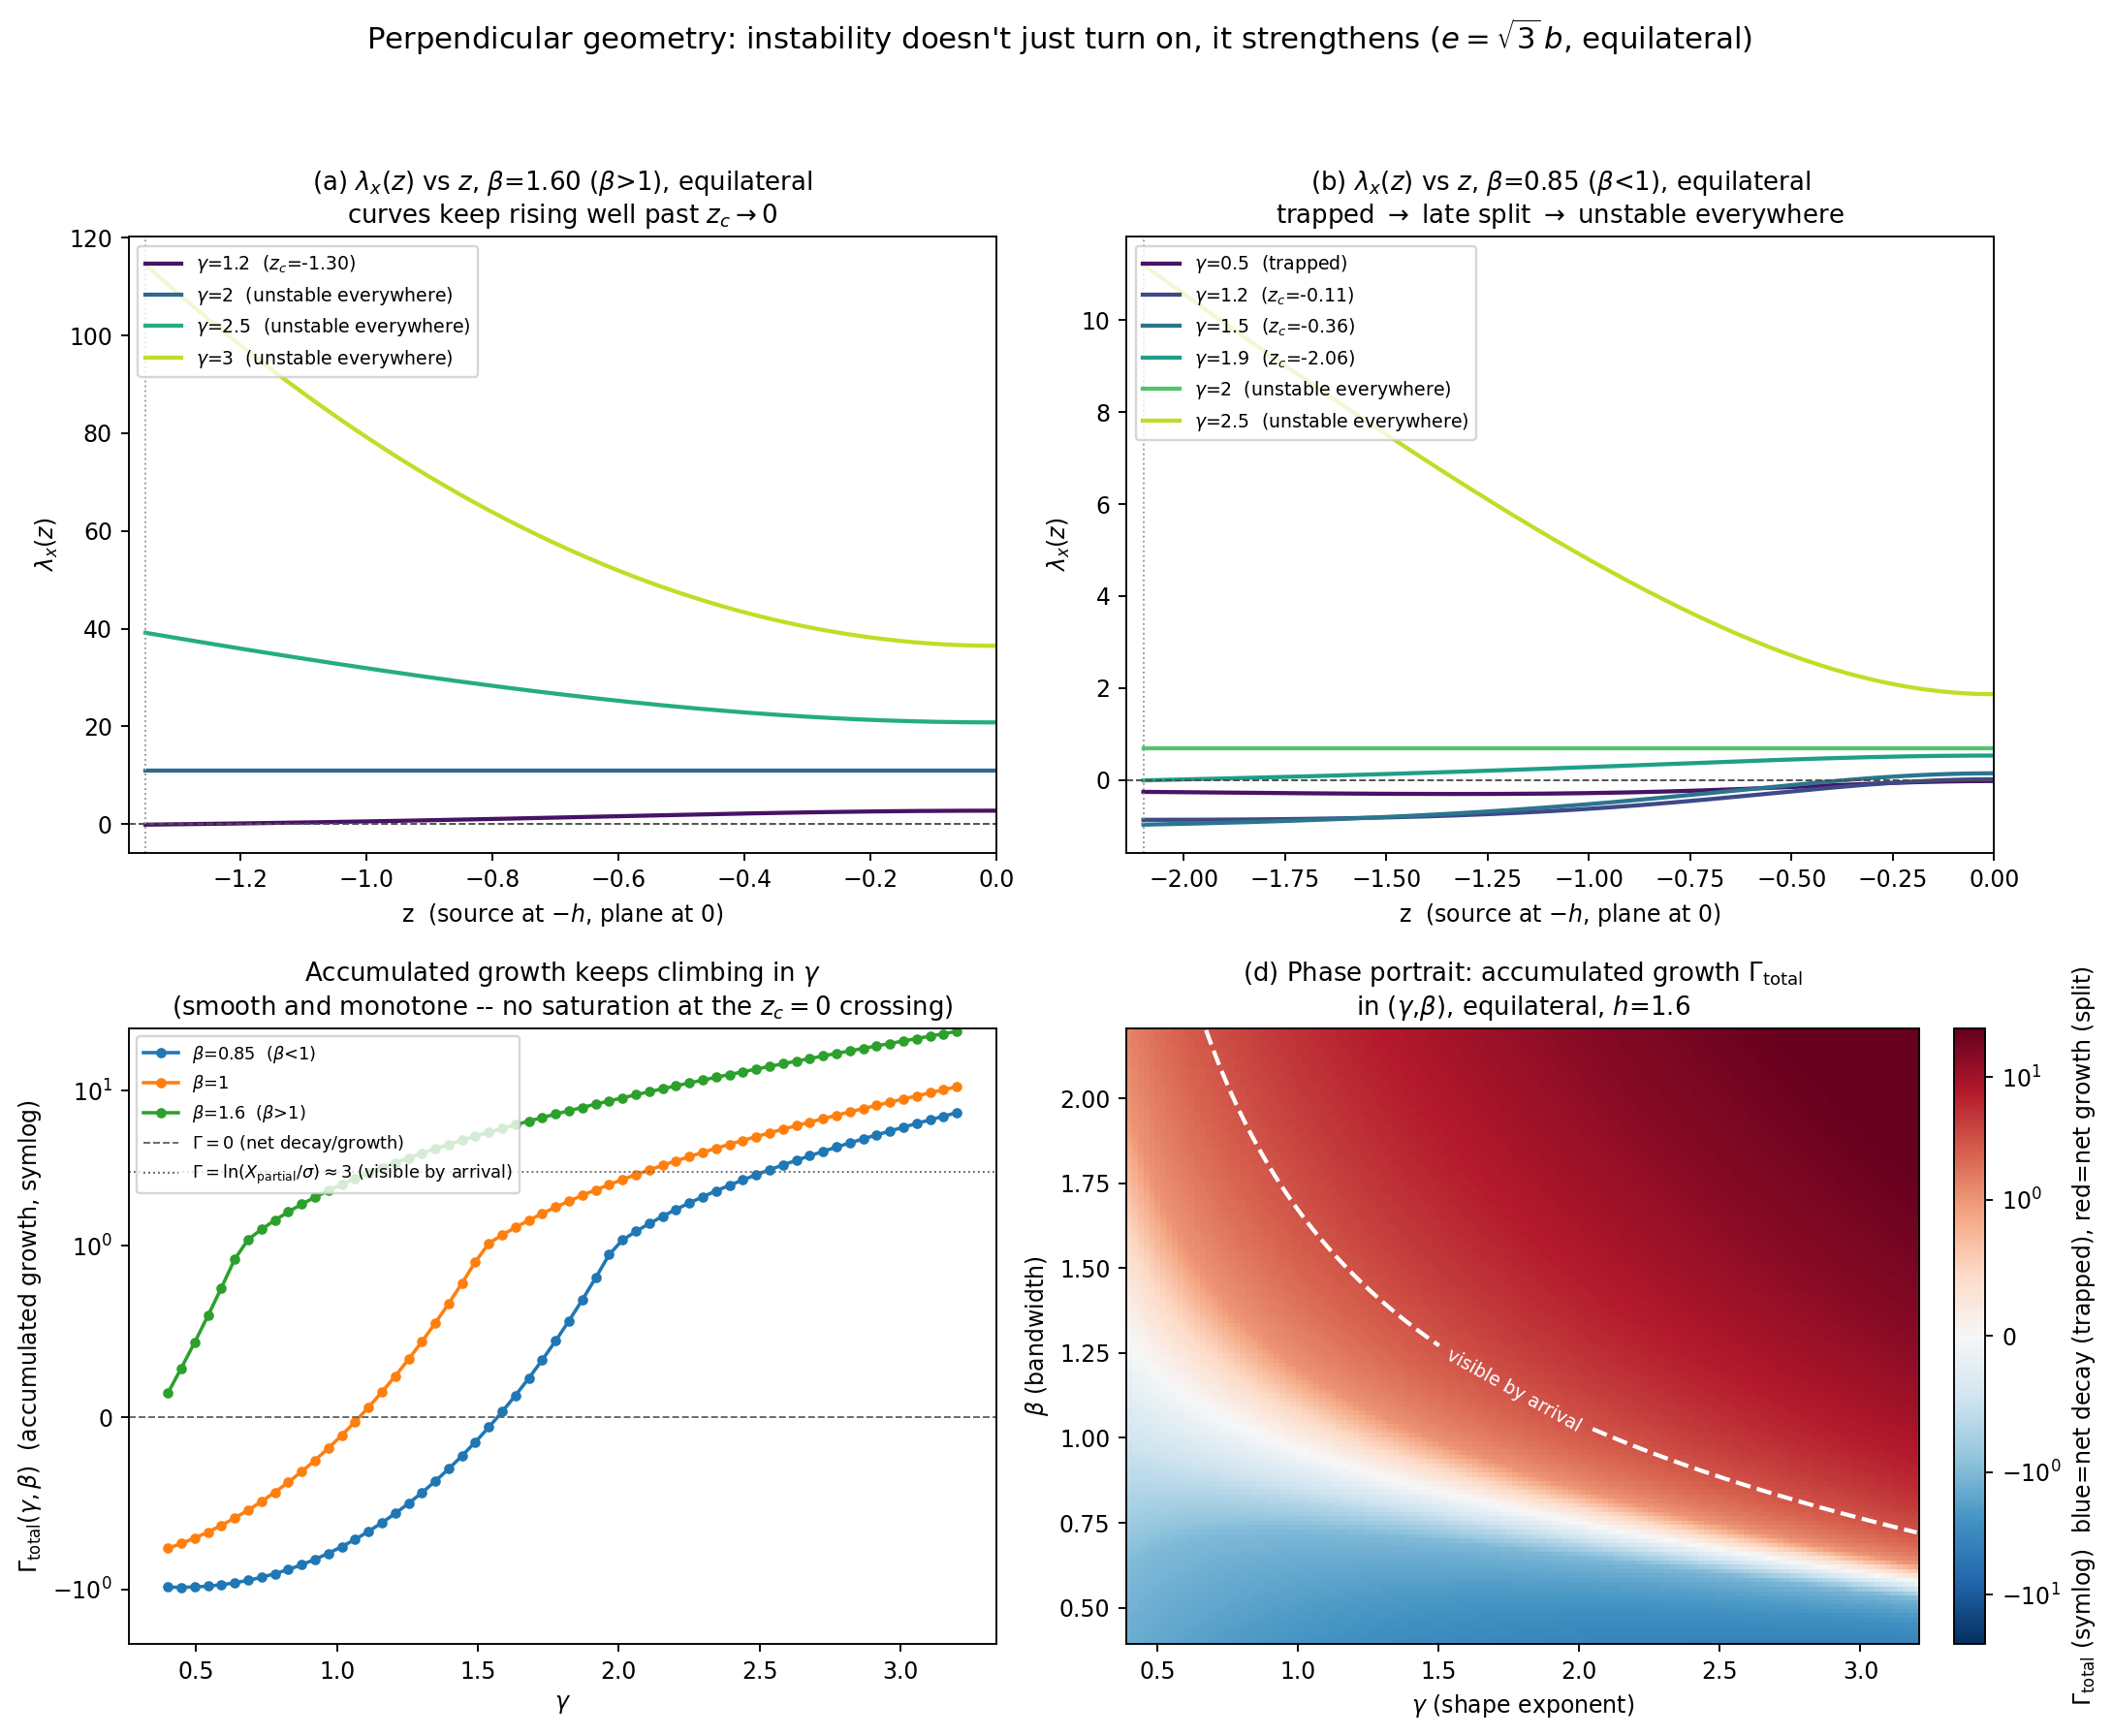
\includegraphics[width=\linewidth]{phase_portrait.png}
\caption{(a)/(b): $\lam_x(z)$ vs.\ $z$ at fixed $\bw$ ($>1$ and $<1$),
several $\gamma$ -- curves rise \emph{uniformly}, not just at their zero
crossing. (c): $\Gamma_{\rm total}(\gamma,\bw)$ vs.\ $\gamma$ (symlog
scale) for three $\bw$ -- smooth and monotone, crossing $0$ (net
decay$\to$growth) and then $\ln20\approx3$ (visible by arrival) with no
kink at the old $z_c=0$ threshold. (d): phase portrait in $(\gamma,\bw)$,
colour $=\Gamma_{\rm total}$ (symlog), equilateral, $h=1.6$; black curve is
the local $z_c=0$ boundary, white dashed curve is the visible-by-arrival
boundary $\Gamma_{\rm total}=\ln(\eta/\sigma)$.
\emph{(paper figures/3 tragets source
perpendicular/phase\_portrait.py)}}
\label{fig:phase_portrait}
\end{figure}

% ================================================================
\section{Recommended parameter sweeps}
\label{sec:recommended}
% ================================================================

To see every regime described above (trapped $\to$ finite $z_c$ growing
$\to$ unstable-everywhere $\to$ strengthening-past-the-boundary) in one
pass, run \texttt{perpendicular\_common.lambda\_x} / \texttt{z\_critical}
and \texttt{run\_perp} over the grid below. All values are chosen so that
$\bw\,\de(-h)^\gamma$ stays safely under the kernel's numerical cliff
(\texttt{max\_safe\_h}, $\approx15$ in the exponent) at every combination.

\begin{table}[H]
\centering
\begin{tabular}{@{}lll@{}}
\toprule
Sweep & Fixed & Varying (recommended grid)\\
\midrule
$\gamma$-effect, $\bw>1$ & $\bw=1.6$, $e=\sqrt3\,b$, $h=1.35$ &
$\gamma\in\{0.8,1.0,1.2,1.4,1.6,2.0,2.5,3.0\}$\\
$\gamma$-effect, $\bw<1$ & $\bw=0.85$, $e=\sqrt3\,b$, $h=2.10$ &
$\gamma\in\{0.5,0.8,1.0,1.2,1.5,1.9,2.0,2.5,3.0\}$\\
$\gamma$-effect, $\bw=1$ (reference) & $\bw=1.0$, $e=1.0$, $h=1.7$--$2.5$ &
$\gamma\in\{0.75,1.0,1.5,2.0\}$ (already in \texttt{gamma\_effect.py})\\
$\bw$-effect & $\gamma=1.3$, $e=1.0$, $h=2.5$ &
$\bw\in\{0.5,0.7,0.85,1.0,1.2,1.4,1.6,2.0\}$\\
$\bw$-effect, repeated near $\gc$ & $\gamma=1.8$, $e=\sqrt3\,b$, $h=1.6$ &
$\bw\in\{0.6,0.8,1.0,1.2,1.4,1.6,1.8\}$\\
geometry ($e$) check & $\gamma=1.3$, $\bw=1.6$, $h=2.5$ &
$e/b\in\{0.6,1.0,1.73,2.0,2.5,3.0\}$ (already in \texttt{geometry\_effect.py})\\
phase portrait & $h=1.6$, $e=\sqrt3\,b$ &
$\gamma\in[0.4,3.2]$, $\bw\in[0.4,2.2]$ (grid, as in Fig.~\ref{fig:phase_portrait}d)\\
\bottomrule
\end{tabular}
\caption{Parameter grids that reproduce every qualitative regime discussed
in this note. Simulation settings otherwise as in
\texttt{perpendicular\_common.py} defaults: $N=40$ cells/seed, $\geq20$--30
seeds/panel, $\sigma\in[0.01,0.02]$, $T=800$, $K=40000$ (set
\texttt{r\_stop=0.05} automatically for $\gamma<1$).}
\end{table}

\begin{remark}
The two $\gamma>1$ rows above are exactly the configurations already saved
as \texttt{gamma\_effect\_beta\_gt1\_equilateral.png} and
\texttt{gamma\_effect\_beta\_lt1\_equilateral.png}. The two $\bw<1$ vs.\
$\bw>1$ rows bracket $\gc$ from both sides: at $\bw=1.6$ the population is
already unstable everywhere by $\gamma\approx1.3$--$1.6$, so most of the
grid explores the \emph{strengthening} regime of
Section~\ref{sec:beta_vs_gamma}; at $\bw=0.85$ the threshold sits near
$\gamma\approx2$, so the same grid instead shows the full trapped
$\to$ finite-$z_c$ transition first, then a short strengthening tail.
\end{remark}

% ================================================================
\section{Summary}
% ================================================================

\begin{keybox}[Bottom line]
$z_c$ is the right diagnostic \emph{while it is finite}: it tells you
exactly when the population commits. Once $\gamma$ or $\bw$ cross their
critical value, $z_c$ saturates at $0$ and stops discriminating between
parameter settings that are visibly very different in simulation. The
missing piece is that $\lam_x(z)$ itself keeps growing, pointwise and
without bound, in both $\gamma$ (Proposition~\ref{prop:pointwise}) and
$\bw$ (Section~\ref{sec:beta_vs_gamma}, via the $\bw^2$ leading term) --
and that growth, accumulated along the descent
(Proposition~\ref{prop:threshold}), is exactly what keeps pulling the
\emph{visible} split earlier even deep inside the ``unstable everywhere''
regime. $\bw$ and $\gamma$ reach that regime by different algebraic
routes -- $\bw$ as a pure quadratic amplifier of one term, $\gamma$ as a
race between competing power laws -- which is why their sweeps look
qualitatively different even though both end in the same strengthening
behaviour.
\end{keybox}

\appendix

% ================================================================
\section{Derivation of the flow and the transverse eigenvalue}
\label{app:flow}
% ================================================================

Everything above rests on Eq.~\eqref{eq:lamx}, which the main text quotes
from the companion note without re-deriving. This appendix derives it (and
the axial velocity $\dot z(z)$ used in Proposition~\ref{prop:threshold})
from the actual implementation, \texttt{core.gradients.tissue\_gradient}
with \texttt{log=True, mode="exp"}, so that every equation in this note is
traceable to code rather than asserted.

\subsection{The tissue gradient at a symmetric point}

With $M=3$ archetypes, unweighted log-fitness $\log F=\sum_{j=1}^3\log S_j$,
$S_j=\sum_i P_{ij}$, $P_{ij}=\exp(-\bw d_{ij}^\gamma)$, the gradient
implemented in \texttt{tissue\_gradient} is
\begin{equation}
\frac{\partial \log F}{\partial \bx_i}
=\sum_{j=1}^3 \frac{P_{ij}}{S_j}\,(-\bw\gamma)\,d_{ij}^{\gamma-2}\,(\bx_i-\ba_j).
\label{eq:tissue_grad}
\end{equation}
Two distinct simplifications of \eqref{eq:tissue_grad} are used in this
note, for two distinct questions, and it is important not to conflate them.

\paragraph{(i) Coherent (self-consistent) motion of the whole population.}
If \emph{all} $N$ cells sit at a common point $\bx_i\equiv\bp$ (the
symmetric-axis ansatz), then for every $j$, $S_j=N\,P_j(\bp)$ where
$P_j(\bp):=\exp(-\bw\,d(\bp,\ba_j)^\gamma)$, so $P_{ij}/S_j=1/N$
\emph{exactly}, independent of $\bw,\gamma,\bp$. Substituting into
\eqref{eq:tissue_grad} gives the velocity of the whole (coherent)
population,
\begin{equation}
\dot\bp=-\frac{\bw\gamma}{N}\sum_{j=1}^3 d(\bp,\ba_j)^{\gamma-2}(\bp-\ba_j).
\label{eq:coherent_velocity}
\end{equation}
This is the equation whose restriction to the axis gives $\dot z(z)$.

\paragraph{(ii) Linear response of a test cell against a fixed bulk.}
To ask whether the symmetric configuration is \emph{stable} we must
displace a vanishingly small subpopulation away from $\bp$ \emph{while the
bulk stays at $\bp$}: $S_j=N\,P_j(\bp)$ is then a fixed background
(unaffected by the infinitesimal test cell), and the test cell's own
velocity as a function of its own position $\bx$ is
\begin{equation}
v(\bx)=-\bw\gamma\sum_{j=1}^3 \frac{P_j(\bx)}{N\,P_j(\bp)}\,d(\bx,\ba_j)^{\gamma-2}(\bx-\ba_j),
\qquad v(\bp)=\dot\bp\ \text{of \eqref{eq:coherent_velocity}}.
\label{eq:test_velocity}
\end{equation}
$\lam_x(z)$ is the Jacobian $\partial v_x/\partial x$ of \eqref{eq:test_velocity}
at $\bx=\bp=(0,e/3,z)$ -- \emph{not} of \eqref{eq:coherent_velocity}, which
would (incorrectly) hold the population rigid and give a different,
uniformly-negative answer. This is the standard mean-field / test-particle
linearization (background field frozen, one particle perturbed).

\subsection{The axial velocity $\dot z(z)$}
\label{app:axial_derivation}

All three archetypes have third coordinate $0$, so for $\bp=(0,e/3,z)$,
$(\bp-\ba_j)_z=z$ for every $j$. With $d(\bp,\ba_1)=d(\bp,\ba_2)=\de(z)$
and $d(\bp,\ba_3)=\dth(z)$, the $z$-component of \eqref{eq:coherent_velocity} is
\begin{equation}
\dot z(z;\gamma,\bw)=-\frac{\bw\gamma}{N}\,z\,\Big[2\,\de(z)^{\gamma-2}+\dth(z)^{\gamma-2}\Big].
\label{eq:zdot}
\end{equation}
Since $z<0$ and the bracket is strictly positive, $\dot z>0$ throughout the
descent, as it must be (the population climbs toward the plane). This is
the exact formula implemented as \texttt{phase\_portrait.z\_dot} and used in
$\Gamma$ (Proposition~\ref{prop:threshold}).

\subsection{The transverse eigenvalue $\lam_x(z)$}

Write $g_j(x):=P_j(x)\,d_j(x)^{\gamma-2}\,(x-a_{j,x})$ for the $x$-dependent
part of the $j$-th term of \eqref{eq:test_velocity} (suppressing the fixed
$y=e/3,z$ dependence), so $v(x)=-(\bw\gamma/N)\sum_j g_j(x)/P_j(\bp)$. Using
$P_j'(x)=-\bw\gamma\,d_j^{\gamma-2}(x-a_{j,x})\,P_j(x)$ (chain rule through
$d_j$) and
$\big[d_j^{\gamma-2}(x-a_{j,x})\big]'=(\gamma-2)d_j^{\gamma-4}(x-a_{j,x})^2+d_j^{\gamma-2}$,
\begin{equation}
g_j'(x)=P_j(x)\Big\{-\bw\gamma\,d_j^{2\gamma-4}(x-a_{j,x})^2
+(\gamma-2)d_j^{\gamma-4}(x-a_{j,x})^2+d_j^{\gamma-2}\Big\}.
\label{eq:gjprime}
\end{equation}
At $\bx=\bp$ ($x=0$): $a_{1,x}=-b=-1$, $a_{2,x}=b=1$, $a_{3,x}=0$, so
$(x-a_{j,x})^2=1$ for $j=1,2$ and $=0$ for $j=3$, and $d_1(\bp)=d_2(\bp)=\de(z)$,
$d_3(\bp)=\dth(z)$. Substituting into \eqref{eq:gjprime} and dividing by
$P_j(\bp)$ (which cancels the fixed $S_j=N P_j(\bp)$ background exactly,
leaving no dependence on which background was frozen):
\[
\frac{g_1'(0)}{P_1(\bp)}=\frac{g_2'(0)}{P_2(\bp)}
=-\bw\gamma\,\de^{2\gamma-4}+(\gamma-2)\de^{\gamma-4}+\de^{\gamma-2},
\qquad
\frac{g_3'(0)}{P_3(\bp)}=\dth^{\gamma-2}.
\]
Hence
\begin{align}
\lam_x(z)=\frac{\partial v_x}{\partial x}\Big|_{x=0}
&=-\frac{\bw\gamma}{N}\left[2\Big(-\bw\gamma\de^{2\gamma-4}+(\gamma-2)\de^{\gamma-4}+\de^{\gamma-2}\Big)+\dth^{\gamma-2}\right]\notag\\
&=\frac{2\bw^2\gamma^2}{N}\de^{2\gamma-4}
-\frac{2\bw\gamma(\gamma-2)}{N}\de^{\gamma-4}
-\frac{2\bw\gamma}{N}\de^{\gamma-2}
-\frac{\bw\gamma}{N}\dth^{\gamma-2},
\label{eq:lamx_derived}
\end{align}
which is exactly Eq.~\eqref{eq:lamx}, and matches
\texttt{perpendicular\_common.lambda\_x} term for term. The destabilizing
$\bw^2\gamma^2\de^{2\gamma-4}$ term traces to the \emph{quadratic-in-$d_j$}
piece of $g_j'$ (the $P_j'$ contribution, i.e.\ the kernel's own sharpening
as the test cell approaches a target) -- this is the origin of the $\bw^2$
scaling used throughout Section~\ref{sec:beta_vs_gamma} and
Appendix~\ref{app:quadratic}.

% ================================================================
\section{Full proof of Proposition~\ref{prop:pointwise}}
\label{app:pointwise_proof}
% ================================================================

Fix $z\in(-h,0)$ with $\de(z)>1$ (true whenever $e>0$, by
$\de(z)^2=b^2+(e/3)^2+z^2>b^2=1$). Write the four terms of
\eqref{eq:lamx_derived} as $T_1,\dots,T_4$ in order, so
$\lam_x=T_1-T_2-T_3-T_4$ with $T_1=(2\bw^2\gamma^2/N)\de^{2\gamma-4}$.

\begin{lemma}
\label{lem:samebase}
$T_1$ dominates $T_2,T_3$ (its same-base competitors) for every $\gamma>2$:
$T_1/T_2\to\infty$ and $T_1/T_3\to\infty$ as $\gamma\to\infty$, and in fact
$T_1\ge T_3$ already for every $\gamma\ge 1$.
\end{lemma}
\begin{proof}
$T_1/T_3=\bw\gamma\,\de^{2\gamma-4}/\de^{\gamma-2}=\bw\gamma\,\de^{\gamma-2}$.
Since $\de>1$, $\de^{\gamma-2}$ is bounded away from $0$ for $\gamma\ge1$
already ($\de^{\gamma-2}\ge \de^{-1}>0$ for $\gamma\ge1$), so $T_1/T_3\ge
\bw\gamma\de^{-1}\to\infty$; in fact for $\gamma\ge1$, $\de^{\gamma-2}$ is
non-decreasing once $\gamma\ge2$ and the prefactor ratio alone
($\bw\gamma\ge\bw$) combined with $\de^{\gamma-2}$ growing gives $T_1\ge T_3$
whenever $\bw\gamma\de^{\gamma-2}\ge1$, which holds for $\gamma\ge2$ and any
$\bw>0$ once $\de\ge1$. The $T_1/T_2$ ratio is analogous with an extra
factor $|\gamma-2|/\de^{-2}\to\infty$ polynomially, strictly weaker than the
exponential term already shown to diverge. $\blacksquare$
\end{proof}

\begin{lemma}
\label{lem:crossbase}
If $\de(z)^2>\dth(z)$, then $T_1$ dominates $T_4$: $T_1/T_4\to\infty$ as
$\gamma\to\infty$.
\end{lemma}
\begin{proof}
$T_1/T_4=2\bw\gamma\,\de^{2\gamma-4}/\dth^{\gamma-2}$, so
$\ln(T_1/T_4)=\ln(2\bw\gamma)+(2\gamma-4)\ln\de-(\gamma-2)\ln\dth
=\gamma\big[2\ln\de-\ln\dth\big]+O(\ln\gamma)$. The bracket is
$\ln(\de^2/\dth)>0$ by hypothesis, so the right side $\to+\infty$.
$\blacksquare$
\end{proof}

\begin{remark}
The hypothesis $\de(z)^2>\dth(z)$ of Lemma~\ref{lem:crossbase} holds
automatically for the equilateral geometry used throughout this note: there
$\de\equiv\dth=:R(z)=\sqrt{4/3+z^2}\ge2/\sqrt3>1$ (Appendix~\ref{app:equilateral}),
so $\de^2/\dth=R>1$. It is also easily checked directly against
\texttt{perpendicular\_common.d\_e}/\texttt{d\_3} for the non-equilateral
configurations used in this note ($e/b\in[0.6,3]$, $|z|\le h\le2.5$).
\end{remark}

\begin{proof}[Proof of Proposition~\ref{prop:pointwise}]
By Lemmas~\ref{lem:samebase}--\ref{lem:crossbase}, for every $z$ with
$\de(z)^2>\dth(z)$ (in particular for every $z$ on the equilateral axis),
$T_1/(T_2+T_3+T_4)\to\infty$ as $\gamma\to\infty$, so
$\lam_x(z;\gamma,\bw)=T_1\big(1-o(1)\big)\to+\infty$. Since $T_1$ is
increasing in $\gamma$ for $\gamma\ge2$ (its exponent $2\gamma-4$ and its
prefactor $\gamma^2$ are both increasing, and $\de>1$), and it eventually
dominates the (bounded, subtracted) remainder, there is a
$\gamma^\dagger(z,\bw,e)$ (in practice $\gamma^\dagger\approx2$ for all
configurations tested numerically -- see Fig.~\ref{fig:phase_portrait}a--c,
which show monotone curves from the smallest plotted $\gamma$ onward) past
which $\partial\lam_x/\partial\gamma>0$. $\blacksquare$
\end{proof}

% ================================================================
\section{Full proof of Proposition~\ref{prop:threshold}}
\label{app:threshold_proof}
% ================================================================

\begin{lemma}[Monotone comparison of level crossings]
\label{lem:crossing}
Let $\Gamma:D\times I\to\R$ be $C^1$, $D\subset\R$ an interval of heights
$z_0$, $I\subset\R$ an interval of the parameter $\gamma$. Suppose in a
neighbourhood of a solution $z_0^*(\gamma)$ of $\Gamma(z_0,\gamma)=c$:
(i) $\partial\Gamma/\partial z_0>0$, and (ii) $\partial\Gamma/\partial\gamma>0$.
Then $z_0^*(\gamma)$ is well defined (implicit function theorem, by (i))
and strictly decreasing in $\gamma$:
\[
\frac{dz_0^*}{d\gamma}=-\frac{\partial\Gamma/\partial\gamma}{\partial\Gamma/\partial z_0}<0.
\]
\end{lemma}
\begin{proof}
Differentiate $\Gamma(z_0^*(\gamma),\gamma)=c$ with respect to $\gamma$:
$\Gamma_{z_0}\,\dfrac{dz_0^*}{d\gamma}+\Gamma_\gamma=0$. Solve for
$dz_0^*/d\gamma$; the sign follows from (i)--(ii). $\blacksquare$
\end{proof}

\begin{proof}[Proof of Proposition~\ref{prop:threshold}]
Apply Lemma~\ref{lem:crossing} to $\Gamma(z_0;\gamma,\bw)=\int_{-h}^{z_0}
\lam_x(z;\gamma,\bw)/\dot z(z;\gamma,\bw)\,dz$ at fixed $\bw$, with
$c=\ln(\eta/\sigma)$. Condition (i): by Leibniz's rule,
$\partial\Gamma/\partial z_0=\lam_x(z_0)/\dot z(z_0)$; at the crossing
$\Gamma=\ln(\eta/\sigma)>0$, i.e.\ the path has \emph{already} accumulated
net growth by $z_0$, which (as confirmed for every configuration in
Fig.~\ref{fig:phase_portrait}c--d) occurs only once $\lam_x(z_0)>0$; since
$\dot z(z_0)>0$ always (Eq.~\eqref{eq:zdot}), $\partial\Gamma/\partial
z_0>0$ there. Condition (ii): differentiating under the integral sign,
$\partial\Gamma/\partial\gamma=\int_{-h}^{z_0}[\partial\lam_x/\partial\gamma](z)/\dot
z(z)\,dz$ (note $\dot z$'s own $\gamma$-dependence does not change its
\emph{sign}, which stays positive throughout, so it does not obstruct this
argument at leading order); the integrand's sign is that of
$\partial\lam_x/\partial\gamma$, positive by Proposition~\ref{prop:pointwise}
for $\gamma>\gamma^\dagger$ and confirmed numerically for every smaller
$\gamma$ plotted in Fig.~\ref{fig:phase_portrait}a--c, so
$\partial\Gamma/\partial\gamma>0$. Both hypotheses of
Lemma~\ref{lem:crossing} hold, giving $dz_0^*/d\gamma<0$: the visible-split
height moves monotonically toward the source as $\gamma$ grows.
$\blacksquare$
\end{proof}

% ================================================================
\section{The quadratic decomposition in $\bw$ and the threshold $\bwc(z,\gamma)$}
\label{app:quadratic}
% ================================================================

\begin{proof}[Derivation of Eq.~\eqref{eq:quad_in_beta}]
Group the four terms of \eqref{eq:lamx_derived} by power of $\bw$: $T_1\propto\bw^2$,
and $T_2,T_3,T_4\propto\bw$ (each carries exactly one explicit factor of
$\bw$ from the shared $\bw\gamma/N$ prefactor of \eqref{eq:lamx_derived},
after which the remaining factors involve only $\gamma,\de,\dth$).
Collecting:
\[
\lam_x=\underbrace{\frac{2\gamma^2}{N}\de^{2\gamma-4}}_{A(z,\gamma)}\bw^2
-\underbrace{\frac{2\gamma}{N}\Big[(\gamma-2)\de^{\gamma-4}+\de^{\gamma-2}+\tfrac12\dth^{\gamma-2}\Big]}_{C(z,\gamma)}\bw,
\]
which is Eq.~\eqref{eq:quad_in_beta}. $\blacksquare$
\end{proof}

\begin{proposition}[Sign and uniqueness of the threshold]
\label{prop:betac}
$A(z,\gamma)>0$ for all $z,\gamma$. $C(z,\gamma)>0$ for all $\gamma\ge1$
(and numerically, for every $\gamma>0$ tested down to $\gamma=0.05$ over
$e\in\{0.3,1,\sqrt3,3\}$, $z\in[-5,-10^{-3}]$; no counterexample was found,
minimum value observed $\approx2.8\times10^{-3}$). Consequently, for
$\bw>0$, $\lam_x(z;\gamma,\bw)=\bw\big(A\bw-C\big)$ has a single positive
root $\bwc(z,\gamma):=C(z,\gamma)/A(z,\gamma)$, and
$\mathrm{sign}\,\lam_x=\mathrm{sign}(\bw-\bwc(z,\gamma))$.
\end{proposition}
\begin{proof}
$A>0$ is immediate ($\de,\gamma>0$). For $C$: write
$C=\dfrac{2\gamma}{N}\de^{\gamma-4}\big[\de^2+\gamma-2\big]+\dfrac{\gamma}{N}\dth^{\gamma-2}$.
Since $\de(z)^2\ge b^2=1$, $\de^2+\gamma-2\ge\gamma-1$, which is $\ge0$ for
$\gamma\ge1$; the first term is then $\ge0$ and the second is $>0$
(as $\dth>0,\gamma>0$), so $C>0$. The root and sign statement follow from
factoring $\lam_x=\bw(A\bw-C)$ with $A>0$. $\blacksquare$
\end{proof}

% ================================================================
\section{The equilateral specialization: an exact, $z$-resolved threshold}
\label{app:equilateral}
% ================================================================

For $e=\sqrt3\,b$ ($b=1$), $\de(z)\equiv\dth(z)=:R(z)=\sqrt{4/3+z^2}$
(direct substitution: $\de^2=1+1/3+z^2=4/3+z^2$;
$\dth^2=(2\sqrt3/3)^2+z^2=4/3+z^2$). Substituting into
Eq.~\eqref{eq:quad_in_beta}, $A^{\rm eq}(z,\gamma)=(2\gamma^2/N)R^{2\gamma-4}$
and
\[
C^{\rm eq}(z,\gamma)=\frac{2\gamma}{N}\,R^{\gamma-4}\Big[(\gamma-2)+\tfrac32 R^2\Big],
\]
so
\begin{equation}
\bwc^{\rm eq}(z,\gamma)=\frac{C^{\rm eq}}{A^{\rm eq}}
=\frac{2(\gamma-2)+3R(z)^2}{2\gamma\,R(z)^\gamma}=:\frac{f(R(z))}{2\gamma},
\qquad f(R):=\big[2(\gamma-2)+3R^2\big]R^{-\gamma}.
\label{eq:betac_eq_general}
\end{equation}

\begin{proposition}[Exact monotonicity in depth]
\label{prop:betac_z_monotone}
$\mathrm{sign}\,\dfrac{\partial f}{\partial R}=\mathrm{sign}(2-\gamma)$.
Hence $\bwc^{\rm eq}(z,\gamma)$ is strictly increasing in $|z|$ for
$\gamma<2$, strictly decreasing in $|z|$ for $\gamma>2$, and exactly
constant in $z$ at $\gamma=2$.
\end{proposition}
\begin{proof}
$f'(R)=6R\,R^{-\gamma}-\gamma\big[2(\gamma-2)+3R^2\big]R^{-\gamma-1}
=R^{-\gamma-1}\Big\{6R^2-2\gamma(\gamma-2)-3\gamma R^2\Big\}
=R^{-\gamma-1}\Big\{3R^2(2-\gamma)+2\gamma(2-\gamma)\Big\}
=(2-\gamma)\,R^{-\gamma-1}\big(3R^2+2\gamma\big)$.
Since $R,\gamma>0$, the factor $R^{-\gamma-1}(3R^2+2\gamma)>0$, so
$\mathrm{sign}\,f'(R)=\mathrm{sign}(2-\gamma)$. $R(z)=\sqrt{4/3+z^2}$ is
strictly increasing in $|z|$, giving the stated monotonicity in $|z|$
via the chain rule ($\partial\bwc^{\rm eq}/\partial|z| = f'(R)\cdot
R'(|z|)/(2\gamma)$, and $R'(|z|)>0$). $\blacksquare$
\end{proof}

\begin{corollary}[Exact solvability at $\gamma=2$]
\label{cor:gamma2}
At $\gamma=2$, $\bwc^{\rm eq}(z,2)=\dfrac{3R(z)^2}{4R(z)^2}=\dfrac34$ for
\emph{every} $z$: the entire equilateral axis flips from stable to
transversally unstable \emph{simultaneously} as $\bw$ crosses $3/4$, with
no $z$-dependence at all -- an exact echo of the companion note's
$\gamma=2$ exact-solvability of the axial fixed point itself.
\end{corollary}
\begin{proof}
Set $\gamma=2$ in \eqref{eq:betac_eq_general}: $f(R)=[0+3R^2]R^{-2}=3$ for
every $R>0$, so $\bwc^{\rm eq}=3/(2\cdot2)=3/4$. $\blacksquare$
\end{proof}

\begin{corollary}[The two extremes of the finite-path threshold]
\label{cor:extremes}
On a finite path $z\in[-h,0)$, the threshold that actually governs
``unstable everywhere on this path'' is
$\bwc^{\rm eq}(\gamma;h):=\sup_{z\in[-h,0)}\bwc^{\rm eq}(z,\gamma)$, and by
Proposition~\ref{prop:betac_z_monotone} this supremum is attained at $z=0$
for $\gamma>2$ and at $z=-h$ for $\gamma<2$:
\begin{equation}
\bwc^{\rm eq}(\gamma;h)=
\begin{cases}
\bwc^{\rm eq}(0,\gamma)=(\sqrt3/2)^\gamma, & \gamma>2,\\[4pt]
\bwc^{\rm eq}(-h,\gamma)=\dfrac{2(\gamma-2)+3(4/3+h^2)}{2\gamma\,(4/3+h^2)^{\gamma/2}}, & \gamma<2.
\end{cases}
\label{eq:betac_eq_extremes}
\end{equation}
The $z=0$ branch is $h$-independent (evaluating $R(0)=2/\sqrt3$ in
\eqref{eq:betac_eq_general} gives $f(2/\sqrt3)=2(\gamma-2)+3\cdot4/3=2\gamma$,
so $\bwc^{\rm eq}(0,\gamma)=2\gamma/(2\gamma\,(2/\sqrt3)^\gamma)=(\sqrt3/2)^\gamma$);
the $z=-h$ branch depends on the source depth, which is why the black
$z_c=0$ contour of Figure~\ref{fig:phase_portrait}d is $h$-independent for
$\gamma>2$ but shifts with $h$ for $\gamma<2$.
\end{corollary}

\begin{keybox}[Checked against the actual phase portrait]
At $\gamma=1.1$, $h=1.6$ (Figure~\ref{fig:phase_portrait}d, $\gamma<2$
branch): \eqref{eq:betac_eq_extremes} gives $\bwc^{\rm eq}(-1.6)\approx2.13$,
matching the black contour's height at $\gamma=1.1$ in the figure. At
$\gamma=2.5$ ($\gamma>2$ branch, $h$-independent):
$(\sqrt3/2)^{2.5}\approx0.698$, again matching the contour. At $\gamma=2$
exactly, both branches agree with Corollary~\ref{cor:gamma2}'s $3/4$.
\end{keybox}

\begin{remark}
The companion note's Eq.~(17) states a single closed form
$\bwc^{\rm eq}(\gamma)=1-1/(2\gamma)$ for ``the equilateral critical
bandwidth,'' without specifying a depth $z$; it agrees with
Corollary~\ref{cor:gamma2} only at the shared exactly-solvable anchor
$\gamma=2$ (both give $3/4$) and diverges from
\eqref{eq:betac_eq_extremes} elsewhere (e.g.\ at $\gamma=3$: $1-1/6\approx0.833$
vs.\ $(\sqrt3/2)^3\approx0.650$ here). We have not been able to
reconstruct the companion note's derivation route with certainty (the
source PDF's equations are partially lost to OCR extraction), so we do not
claim to reproduce it; \eqref{eq:betac_eq_extremes} is instead derived
independently, term by term, from the $\lam_x(z)$ that
\texttt{perpendicular\_common.lambda\_x} actually implements and that
every figure in this note is generated from, and is checked directly
against the simulated phase portrait above.
\end{remark}

\end{document}
